%%%%%%%%%%%%%%%%%%%%%%%%%%%%%%%%%%%%%%%%%%%%%%%%%%%%%%%%%%%%%%%%%%%%%%%%%%%%%%%%%
%
%  Vishnudev Krishnadas Vishnudev Krishnadas 17.04.2023         
%  "Self-supervised Learning for different Downstream Tasks"
%  Lehrstuhl fuer Mustererkennung, FAU Erlangen-Nuernberg
%
%%%%%%%%%%%%%%%%%%%%%%%%%%%%%%%%%%%%%%%%%%%%%%%%%%%%%%%%%%%%%%%%%%%%%%%%%%%%%%%%%

% Document class for LME theses: lmedoc
% %LANGUAGE
% %CONFIG
%    The option "german" uses german.sty
%    For english papers, use the "english" option
% Possible types of theses:
% bt - Bachelor's thesis
% mt - Master's thesis
% diss - Dissertation
% sa - Student thesis
% mp - Master Project
%\documentclass[german,bt]{lmedoc/lmedoc}
\documentclass[english,mp]{lmedoc/lmedoc-ai}

\usepackage[skip=6pt, indent=40pt]{parskip}

%%%%%%%%%%%%%%%%%%
% pdflatex and lualatex are supported
% ++ "Umlaut" support
%    The package "inputenc" can be used to write Umlaute or the german double s
%    directly. You need to use the correct encoding, e.g. latin1.
\usepackage{iftex}
\ifPDFTeX
  \usepackage[utf8]{inputenc}
  \usepackage[T1]{fontenc}
  \usepackage{lmodern}
\else
  \ifXeTeX
     \usepackage{fontspec}
  \else 
     \usepackage{luatextra}
  \fi
\fi

%%%%%%%%%%%%%%%%%%
% ++ use \toprule,\midrule und \endrule in your tables, no \hline or vertical
% columns please
\usepackage{booktabs}
% guessing if space is needed
\usepackage{xspace}

% mathstuff
\usepackage{amsmath,amssymb}
\usepackage{mathtools}
\usepackage{bm}

% Color stuff
\usepackage[usenames,dvipsnames,table]{xcolor}
% let's define a dark blue color
\definecolor{faublue}{RGB}{0,51,102}

% Images
\usepackage{graphicx}
\graphicspath{ {./images} }


% defines units
\usepackage[binary-units,abbreviations]{siunitx}

% allows inline enumerate
\usepackage[inline]{enumitem}
% and sets them to Arabic
\setlist*[enumerate]{label=(\arabic*)}
% remove widows at end or beginning of a page
\usepackage[all]{nowidow}

% great packages to make nice figures/plots/ 
\usepackage{tikz}
%\usepackage{pgfplots}

% you can even separate table content and layout
%\usepackage{pgfplotstable} 
%\pgfplotsset{compat=newest}

% url package, it also breaks at hyphens
\usepackage[hyphens]{url}

% typesetting numbers and units
\usepackage{siunitx}
\sisetup{mode=text}% use text mode for numbers

% ++ \url{} better breaking of urls and connect w. hyperref
\usepackage{url}
% ++ Biblatex
%    Replaces the old 'bibtex'. The bibtex step has to be replaced with 'biber'.
\usepackage[backend=biber, bibencoding=utf8, giveninits=true,
maxbibnames=99, % show all authors in the bibliography
maxalphanames=1, minalphanames=1, style=alphabetic,%
style=trad-alpha, backref=true]{biblatex}
% biblatex backref
\DefineBibliographyStrings{english}{%
  backrefpage = {cited on p\onedot},
	backrefpages = {cited on pp\onedot},
}

% ++ use for refercence farther away: \vref
\usepackage{varioref}
\renewcommand\reftextfaraway[1]{(p.\,\pageref{#1})}
% ++ Makes all the references in the document clickable.
%    To ensure that backref is working, this package has to be loaded after biblatex.
\usepackage{hyperref}
\hypersetup{
  colorlinks = true,   % Führt zu einem farbigen Ausdruck!
  linkcolor =  faublue,
  urlcolor =   magenta,
  citecolor =  faublue,
  plainpages =        false,
  hypertexnames =     true,
  linktocpage =       true,
  bookmarksopen =     true,
  bookmarksnumbered = true,
  bookmarksopenlevel= 0,
% pdf information, uncomment if done
%  pdftitle =    {your thesis title},
%  pdfauthor =   {your name},
%  pdfsubject =  {Master's thesis},
%  pdfkeywords = {put in some comma-separated keywords}
}
% Enable correct jumping to figures when referencing
\usepackage[all]{hypcap}

% ++ use for refercence in the local arae \cref, e.g. \cref{fig:xyz}
%  has to come after hyperref package
\usepackage[noabbrev,capitalise,nameinlink]{cleveref}


% ++ use multiple figures/tables in one
\usepackage{caption}
\usepackage{subcaption}
\captionsetup[table]{position=top}
\captionsetup[figure]{position=bottom}
% \captionsetup[subtable]{position=bottom}
% will result in references (typeset with \ref )
% like ‘1a’ but sub-references (typeset with \subref) like ‘(a)’.
\captionsetup{subrefformat=parens}


% ++ Enables glossaries-extra. Should be used for abbreviations in the paper.
\usepackage[abbreviations,shortcuts=true,nogroupskip]{glossaries-extra}
% abbreviationstyle for acronyms
\setabbreviationstyle{long-short}
% one can also use \makeglossaries and \printglossaries however then you need to
% create a latexmk file and it might become more complicated for Windows users...

% put in this file your abbreviations
% add your abbreviations here
\newacronym{icdar}{ICDAR}{International Conference on Document Analysis}
\newacronym{clamm}{CLaMM}{Classification of Latin Medieval Manuscripts}
\newacronym{ssl}{SSL}{Self-supervised Learning}
\newacronym{simclr}{SimCLR}{Simple Framework for Contrastive Learning of Visual Representations}
\newacronym{mae}{MAE}{Masked Autoencoders}
\newacronym{byol}{BYOL}{Bootstrap Your Own Latent}
\newacronym{vit}{ViT}{Vision Transformer}
\newacronym{tsne}{t-SNE}{t-distributed Stochastic Neighbor Embedding}
\newacronym{gpu}{GPU}{Graphics Processing Unit}
\newacronym{slurm}{SLURM}{Slurm Workload Manager}
\newacronym{nan}{NaN}{Not a Number}
%%%%%%%%%%%%%%%%%%%%%%%%%%%%

% supress messages because of underful hbox, this is not a problem
\hbadness=10000



% some useful commands
\makeatletter % let's define a single dot
\DeclareRobustCommand\onedot{\futurelet\@let@token\@onedot}
\newcommand{\@onedot}{\ifx\@let@token.\else.\null\fi\xspace}
\makeatother

\newcommand{\etal}[1]{#1~et~al\onedot}
\def\accto{acc.~to\xspace}
\newcommand{\eg}{e.\,g.,\xspace}
\newcommand{\Eg}{E.\,g.,\xspace}
\newcommand{\cf}{cf\onedot}
\newcommand{\ie}{i.\,e.,\xspace}
\newcommand{\wrt}{w.\,r.\,t\onedot}
\newcommand{\aka}{a.\,k.\,a\onedot}
\newcommand{\todo}[1]{\textcolor{red}{TODO: #1}}
\renewcommand{\vec}[1]{\bm{#1}}


% Sets the bib file

\addbibresource{literature.bib}

% When writing a large document, it is sometimes useful to work on selected sections of the document.
% Use this command to only build the document partially. Speeds up the developement cycle.
% For the final product, this has to be commented out.
%\includeonly{introduction,appendix,foo,bar}


\pagenumbering{roman}

\begin{document}
\clearpage
% %CONFIG
% This is for students' master project
\begin{deckblatt}
\Titel{Self-supervised Learning for different Downstream Tasks} % Title
\Name{Vishnudev Krishnadas} % Last name
\Vorname{Vishnudev Krishnadas} % Given name
\Geburtsort{Kerala, India} % Place of birth
\Geburtsdatum{24.02.1997} % Date of birth
\Betreuer{Dr.-Ing. Vincent Christlein} % Advisor
% \Start{01.11.2022} % Start of thesis
% \Ende{Ende} % End of thesis
%\ZweitInstitut{ZweitInstitut} % Cooperation partner
\end{deckblatt}


% \cleardoublepage


% Ich versichere, dass ich die Arbeit ohne fremde Hilfe und ohne Benutzung
% anderer als der angegebenen Quellen angefertigt habe und dass die Arbeit
% in gleicher oder "ahnlicher Form noch keiner anderen Pr"ufungsbeh"orde
% vorgelegen hat und von dieser als Teil einer Pr"ufungsleistung
% angenommen wurde. Alle Ausf"uhrungen, die w"ortlich oder sinngem"a"s
% "ubernommen wurden, sind als solche gekennzeichnet.
% \\

% Die Richtlinien des Lehrstuhls f"ur Studien- und Diplomarbeiten
% habe ich gelesen und anerkannt, insbesondere die Regelung des
% Nutzungsrechts. \\[15mm]
% Erlangen, den {\selectlanguage{german} \today} \hspace{6.0cm} \\[10mm] 



% \cleardoublepage


% \begin{center}
% \bfseries
% % Abstract in German
% {\selectlanguage{german}"Ubersicht}
% \normalfont
% \end{center}


% \vspace{5.0cm}

\begin{center}
\bfseries
% Abstract in English
{\selectlanguage{english}Abstract}
\normalfont
\end{center}

%%%%%%%%%%%%%%%%%%%%%%%%%
% ABSTRACT
%%%%%%%%%%%%%%%%%%%%%%%%%

This project presents a comparison of self-supervised learning methods for different downstream tasks in the context of Medieval Handwriting in the Latin Script dataset. Self-supervised learning has shown promise in various computer vision and natural language processing applications, but its effectiveness on historical scripts has not been extensively explored. Three self-supervised learning methods, namely, \gls{simclr}, \gls{mae}, and \gls{byol} are compared in this work. The performance evaluation was conducted on one downstream tasks i.e. script type classification. The results indicate that the \gls{simclr} method outperforms other methods in the downstream task for the Medieval Handwritings Script dataset. Additionally, insights were provided regarding the factors influencing the performance of self-supervised learning methods in this context, including the selection of pre-training data and the size of the pre-training dataset. In conclusion, this study showcases the potential of self-supervised learning for historical handwritten document classification tasks and emphasizes the significance of selecting suitable methods for specific downstream tasks.


%%%%%%%%%%%%%%%%%%%%%%%%%

\tableofcontents

\pagenumbering{arabic}

\chapter{Introduction}

The increasing digitization of historical documents has created demand for efficient and accurate methods to categorize and organize these valuable ancient scripts. The field of Deep Learning has met with great success in many problems involving complex data \cite{najafabadi_deep_2015}. The majority of the available digitized corpus is unlabeled and lacks metadata. Consequently, an unsupervised approach to learning is necessary which takes advantage of the large amounts of unlabeled data. Hence, this master project evaluates the efficacy of Deep Learning based Self-supervised Learning approaches in the context of historical documents. Self-supervised learning models extract intrinsic patterns from the data, which is used for knowledge transfer to the target task.

This project focuses on the style classification of Medieval Handwritings in Latin Script and is the target task in this work. Style classification may also be referred to as script type classification in this report. The Script type classification refers to the task of categorizing Latin scripts according to morphological differences in the handwritten text \cite{cloppet_icdar2017_2017}. Representations produced by the self-supervised model are employed to enhance the accuracy of script type prediction by utilizing the morphology present in the text. For this study, it was of interest to investigate \acrfull{simclr} \cite{chen_simple_2020}, \acrfull{mae} \cite{he_masked_2021}, and \acrfull{byol} \cite{grill_bootstrap_2020} \acrfull{ssl} methods. The scope of this project is to compare the quality of generated representations by the mentioned self-supervised learning techniques.

The upcoming chapters of this study will consist of an overview of the dataset and the self-supervised algorithms employed. In addition, the methods utilized will be carefully examined. Subsequently, the results and analysis of the study will be presented.

% % let's show you how \cite and \gls for abbreviations works
% Example paragraph: 

% Useful reads:

% Checkout the subcaption package how to do multiple figures/tables. Make sure
% that you use vector graphics - no blurry png - for graphs or similar, \eg use
% tikz/inkscape. \cref{fig:ex} is an example of a figure using the package tikz. Make also sure that your plots are readable and have axis
% captions, \eg use pgfplots.

% How to create good looking tables with the booktabs package
% e.g. a table should like \cref{tab:ex}.

% \begin{table}
%     \centering
%         \caption[Short title for the List of Tables.]{Long caption for this table which is composed by sub-table 1 and sub-table 2.}
%         \begin{subtable}{.5\textwidth}
%             \centering
%                 \caption{Sub-table 1.}
%             	\begin{tabular}{llr}
%             		\toprule
%             		id & method & result\\
%             		\midrule
%             		1 & A & 0.9\\
%             		2 & B & 0.8\\
%             		\bottomrule
%             	\end{tabular}
%         \end{subtable}% <---- don't forget this %
%         \begin{subtable}{.5\textwidth}
%             \centering
%                 \caption{Sub-table 2.}
%             	\begin{tabular}{llr}
%             		\toprule
%             		id & method & result\\
%             		\midrule
%             		1 & C & 90\%\\
%             		2 & D & 80\%\\
%             		\bottomrule
%             	\end{tabular}
%         \end{subtable}
% \label{tab:ex}
% \end{table}


% \begin{figure}
% \centering
%  \centering
 \begin{tikzpicture}[scale=0.5]
  \node[draw] at (3,7) {Generative};

  \draw[draw=red,fill=red] (1,1) circle (0.2);
  \draw[draw=red,fill=red] ( 2 , 3.5 ) circle (0.2);
  \draw[draw=red,fill=red] ( 0 , 3 ) circle (0.2);
  \draw[draw=red,fill=red] ( 1 , 2 ) circle (0.2);
  \draw[draw=red,fill=red] ( 2 , 3 ) circle (0.2);
  \draw[draw=red,fill=red] ( 3 , 1 ) circle (0.2);
  \draw[draw=red,fill=red] ( 1 , 4 ) circle (0.2);
  \draw[draw=red,fill=red] (1.8,2.5) circle (0.2);
  %
  \draw[rotate around={35:(2,2)},fill=red, opacity=0.2] (1.8,2.5) ellipse (1.5 and 2.5);
  \draw[rotate around={35:(2,2)},fill=red, opacity=0.21] (1.8,2.5) ellipse (1.2 and 2.2);
  \draw[rotate around={35:(2,2)},fill=red, opacity=0.22] (1.8,2.5) ellipse (0.9 and 1.9);
  %%%%%%%%%%%%%%%%%%%%%
  \draw[draw=cyan,fill=cyan] ( 4 , 3 ) circle (0.2);
  \draw[draw=cyan,fill=cyan] ( 4 , 4 ) circle (0.2);
  \draw[draw=cyan,fill=cyan] ( 5 , 5 ) circle (0.2);
  \draw[draw=cyan,fill=cyan] ( 5 , 3 ) circle (0.2);
  \draw[draw=cyan,fill=cyan] ( 3 , 4 ) circle (0.2);
  \draw[draw=cyan,fill=cyan] ( 3 , 5 ) circle (0.2);
  \draw[draw=cyan,fill=cyan] ( 5 , 3 ) circle (0.2);
  \draw[rotate around={35:(4.5,4)},fill=cyan, opacity=0.2] (4.3,4.2) ellipse (1.5 and 1.8);
  \draw[rotate around={35:(4.5,4)},fill=cyan, opacity=0.21] (4.3,4.2) ellipse (1.2 and 1.5);
  \draw[rotate around={35:(4.5,4)},fill=cyan, opacity=0.22] (4.3,4.2) ellipse (0.9 and 1.2);
  %%%%%%%%%%%%%%%%%%%%%%%%%%%%%%%%%%%%%%%%%
  \node[draw] at (13,7) {Discriminative};
  \draw[ultra thick] (15,0) -- (11,6cm);
  \draw[draw=red,fill=red] ( 11 , 1 ) circle (0.2);
  \draw[draw=red,fill=red] ( 12, 3.5) circle (0.2);
  \draw[draw=red,fill=red] ( 10 , 3 ) circle (0.2);
  \draw[draw=red,fill=red] ( 11 , 2 ) circle (0.2);
  \draw[draw=red,fill=red] ( 12 , 3 ) circle (0.2);
  \draw[draw=red,fill=red] ( 13 , 1 ) circle (0.2);
  \draw[draw=red,fill=red] ( 11 , 4 ) circle (0.2);
  \draw[draw=red,fill=red] (11.8,2.5) circle (0.2);
  %%%%%%%%%%%%%%%%%%%%%
  \draw[draw=cyan,fill=cyan] ( 14 , 3 ) circle (0.2);
  \draw[draw=cyan,fill=cyan] ( 14 , 4 ) circle (0.2);
  \draw[draw=cyan,fill=cyan] ( 15 , 5 ) circle (0.2);
  \draw[draw=cyan,fill=cyan] ( 15 , 3 ) circle (0.2);
  \draw[draw=cyan,fill=cyan] ( 13 , 4 ) circle (0.2);
  \draw[draw=cyan,fill=cyan] ( 13 , 5 ) circle (0.2);
  \draw[draw=cyan,fill=cyan] ( 15 , 3 ) circle (0.2);
 \end{tikzpicture}
% \caption{Example of a figure using the package \textit{tikz}}
% \label{fig:ex}
% \end{figure}
   % Introduction 

\chapter{Materials and Methods}
Self-supervised representation learning is used to obtain visual features from a large scale of unlabeled data. These visual features are discovered by learning the objective function of a pretext task. To assess the quality of features generated by the pretext task, a downstream task based on an application is selected. Knowledge transfer from the pre-trained model in the pretext task proves valuable for the downstream or target task \cite{ericsson_self-supervised_2022}. In this project, the target task is defined as script-type classification for Medieval Latin scripts.

\section{Dataset}

The dataset used in this project comes from the \acrfull{icdar} 2017 competition on the \acrfull{clamm} \cite{cloppet_icdar2017_2017}. All self-supervised models used were pre-trained on a dataset with 70\% of 5,540 images combining the \textit{Training dataset} and \textit{Tasks 1 \& 3 dataset} provided on the competition portal \cite{noauthor_icdar2017-clamm_nodate}. Then, a linear evaluation protocol was followed to evaluate the model's performance and compare it with other models. The subsequent sections detail the setup for the state-of-the-art \gls{ssl} methods used in this project.

\section{Software and Hardware environment}

All the methods were implemented with Pytorch Lightning \cite{Falcon2019} and the Hydra framework \cite{Yadan2019Hydra} for configurations and experiments. The experiments were executed on a High Performance Cluster with \glspl{gpu} using \gls{slurm} jobs. The \glspl{gpu} used for pre-training were Nvidia GeForce RTX3080 and Nvidia A100 Tensor Core.

\section{Self-supervised learning techniques}

\subsection{Simple Framework for Contrastive Learning of Visual Representations}

\gls{simclr} has garnered considerable attention in the machine learning community due to its efficacy in learning meaningful representations from unlabeled data. The \gls{simclr} architecture comprises several key components: a data augmentation module, a base encoder (ResNet-50), a compact projection head, and a contrastive loss function \cite{chen_simple_2020}. In the following discussion, we delve into the configuration of these components.

\begin{itemize}

\item{\textbf{Data augmentation}} module plays a pivotal role and encompasses a sequential series of transformations applied probabilistically. These transformations include random resized crop, horizontal flip, gaussian blur, random rotation, random erasing, dilation, erosion, and normalization. By simulating various nuances found in historical handwritten documents — such as smudging, ink bleeding, discoloration, folds, stains, and others — the augmentations contribute significantly to the model's generalization capabilities.

\item{\textbf{Backbone architecture.}} In order to extract representations from the augmented data, the ResNet-50 neural network encoder architecture is employed. This architecture has been proven effective in capturing relevant features from the input data.

\item{\textbf{Projection head}} serves as a crucial component responsible for reducing the dimensionality of the data. It consists of a sequential neural network comprising two linear layers, with batch normalization and ReLU activation applied in between. This configuration enables the projection head to extract compact representations from the higher-dimensional space.

\item{\textbf{Loss function.}} As recommended by Ting Chen et al. \cite{chen_simple_2020}, the Normalized Temperature-scaled Cross Entropy Loss is employed as the contrastive loss function. This loss function aids in maximizing agreement between differently augmented views of the same sample while minimizing agreement between views of different samples.

\end{itemize}

\begin{figure}[ht]
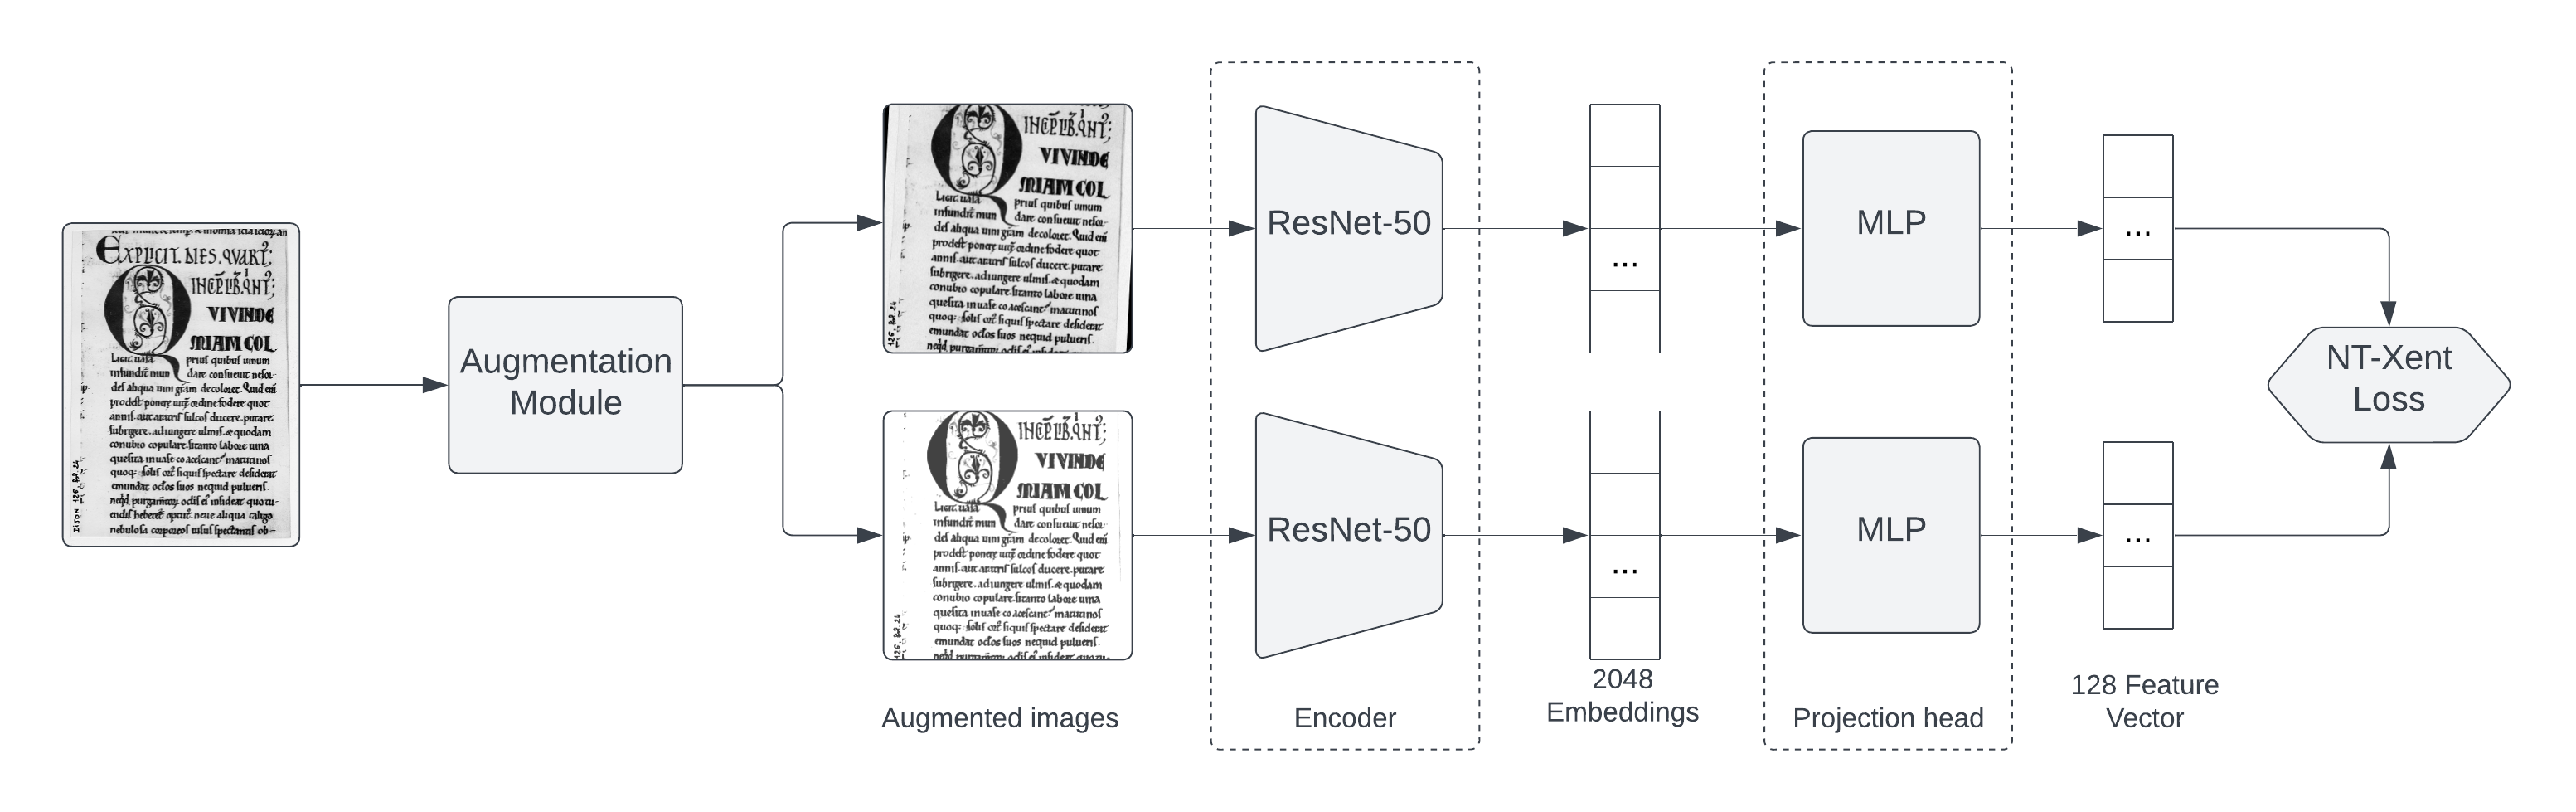
\includegraphics[width=\textwidth]{simclr_arch.png}
\centering
\caption{SimCLR Architecture}
\label{fig:figure}
\end{figure}

\subsection{Masked Autoencoders}
\gls{mae} can serve as powerful pretraining models for deep neural networks. By training an autoencoder on a large unlabelled dataset, it can learn general features or representations that capture the statistical regularities of the data. \gls{mae} comprise two key components: an encoder consisting of \acrfull{vit} blocks in series and a lightweight decoder that reconstructs the input from the representation generated by the encoder. Another essential technique included is an optimal masking ratio of 75\% to balance the accuracy and generalization of the model \cite{he_masked_2021}.

A set of five \gls{vit} architecture sizes from ViT-Tiny to ViT-Huge were evaluated for the encoder. The encoder operates on a visible subset of patches without the mask tokens and a shallow decoder reconstructs the original image from the representation generated by the encoder. Simple transformations of resize, crop and flip are applied. Xavier Uniform technique is used to initialize the weights for all the transformer blocks. The mean squared error at the pixel level between the input and the reconstructed image is used as the loss. 

\begin{figure}[ht]
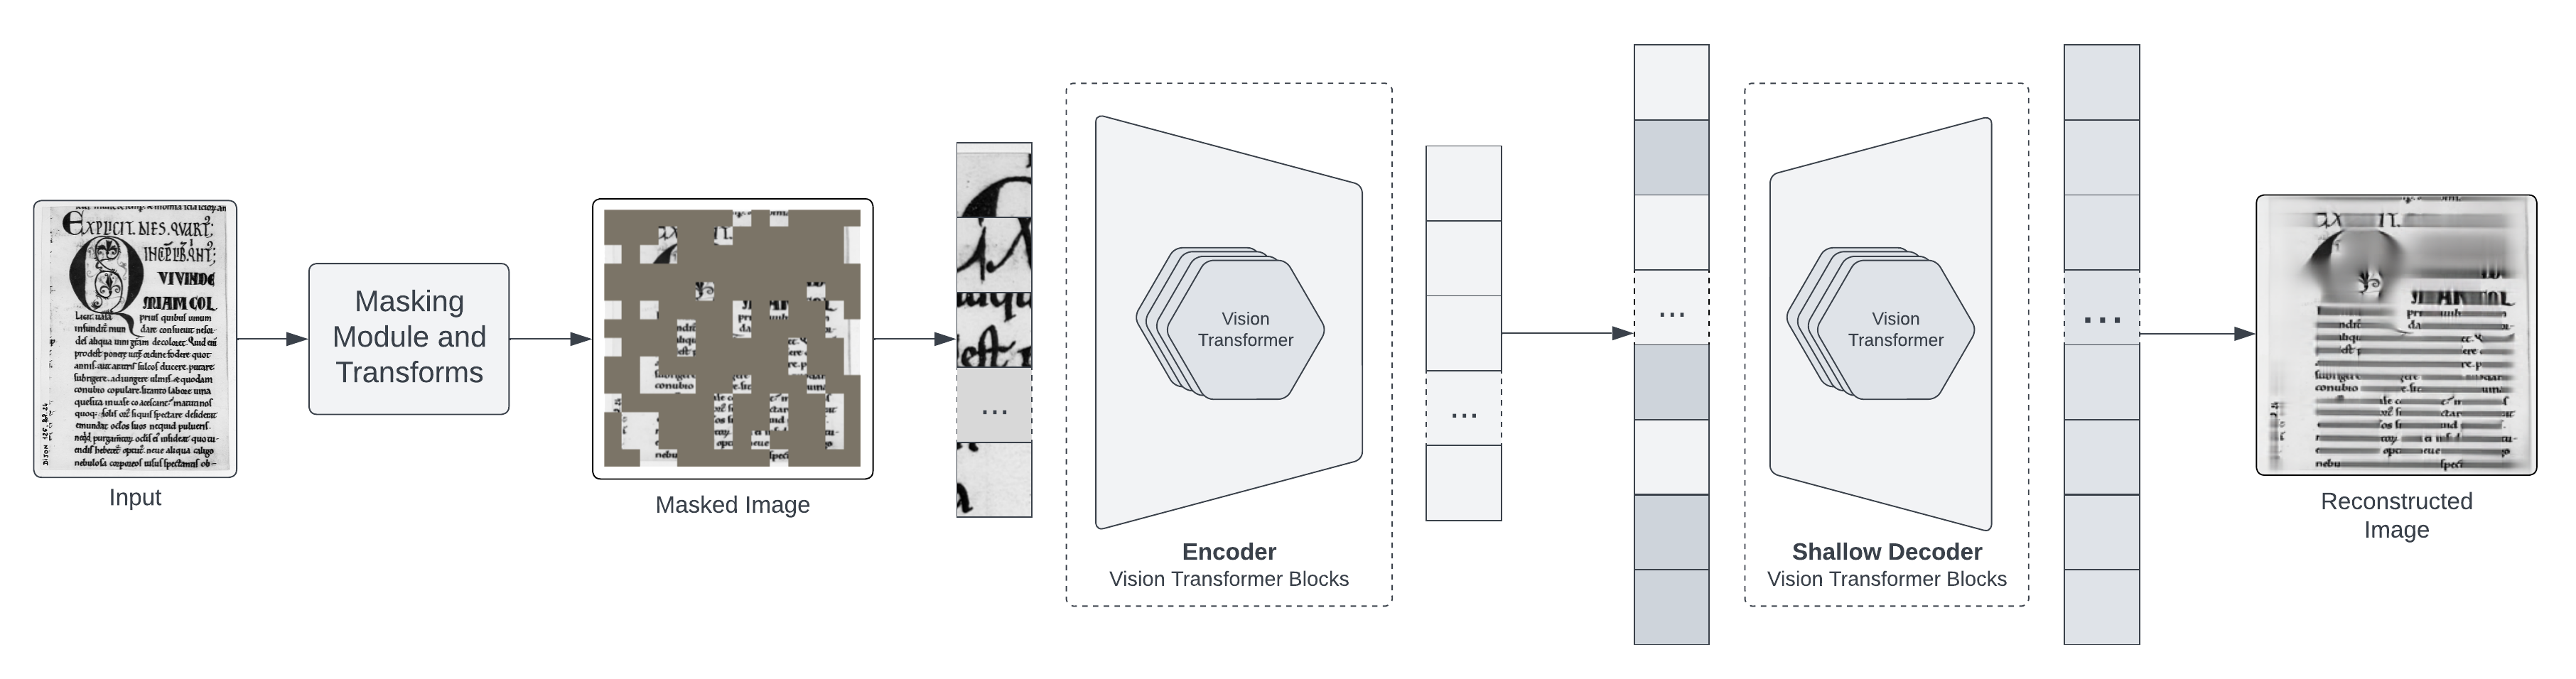
\includegraphics[width=\textwidth]{mae_arch.png}
\centering
\caption{MAE Architecture}
\label{fig:figure}
\end{figure}

\subsection{Bootstrap Your Own Latent}

\gls{byol} uses two neural networks, referred to as the online and target networks, which work together to learn from one another. Both the networks use a ResNet-50 architecture as the backbone and a multi-layer perceptron as the projection network. Additionally, a cosine based similarity loss between the online and target networks plays a vital role in effective learning \cite{grill_bootstrap_2020}. The augmentations for images in the online and target networks are the same as in \gls{simclr}. 

\begin{figure}[ht]
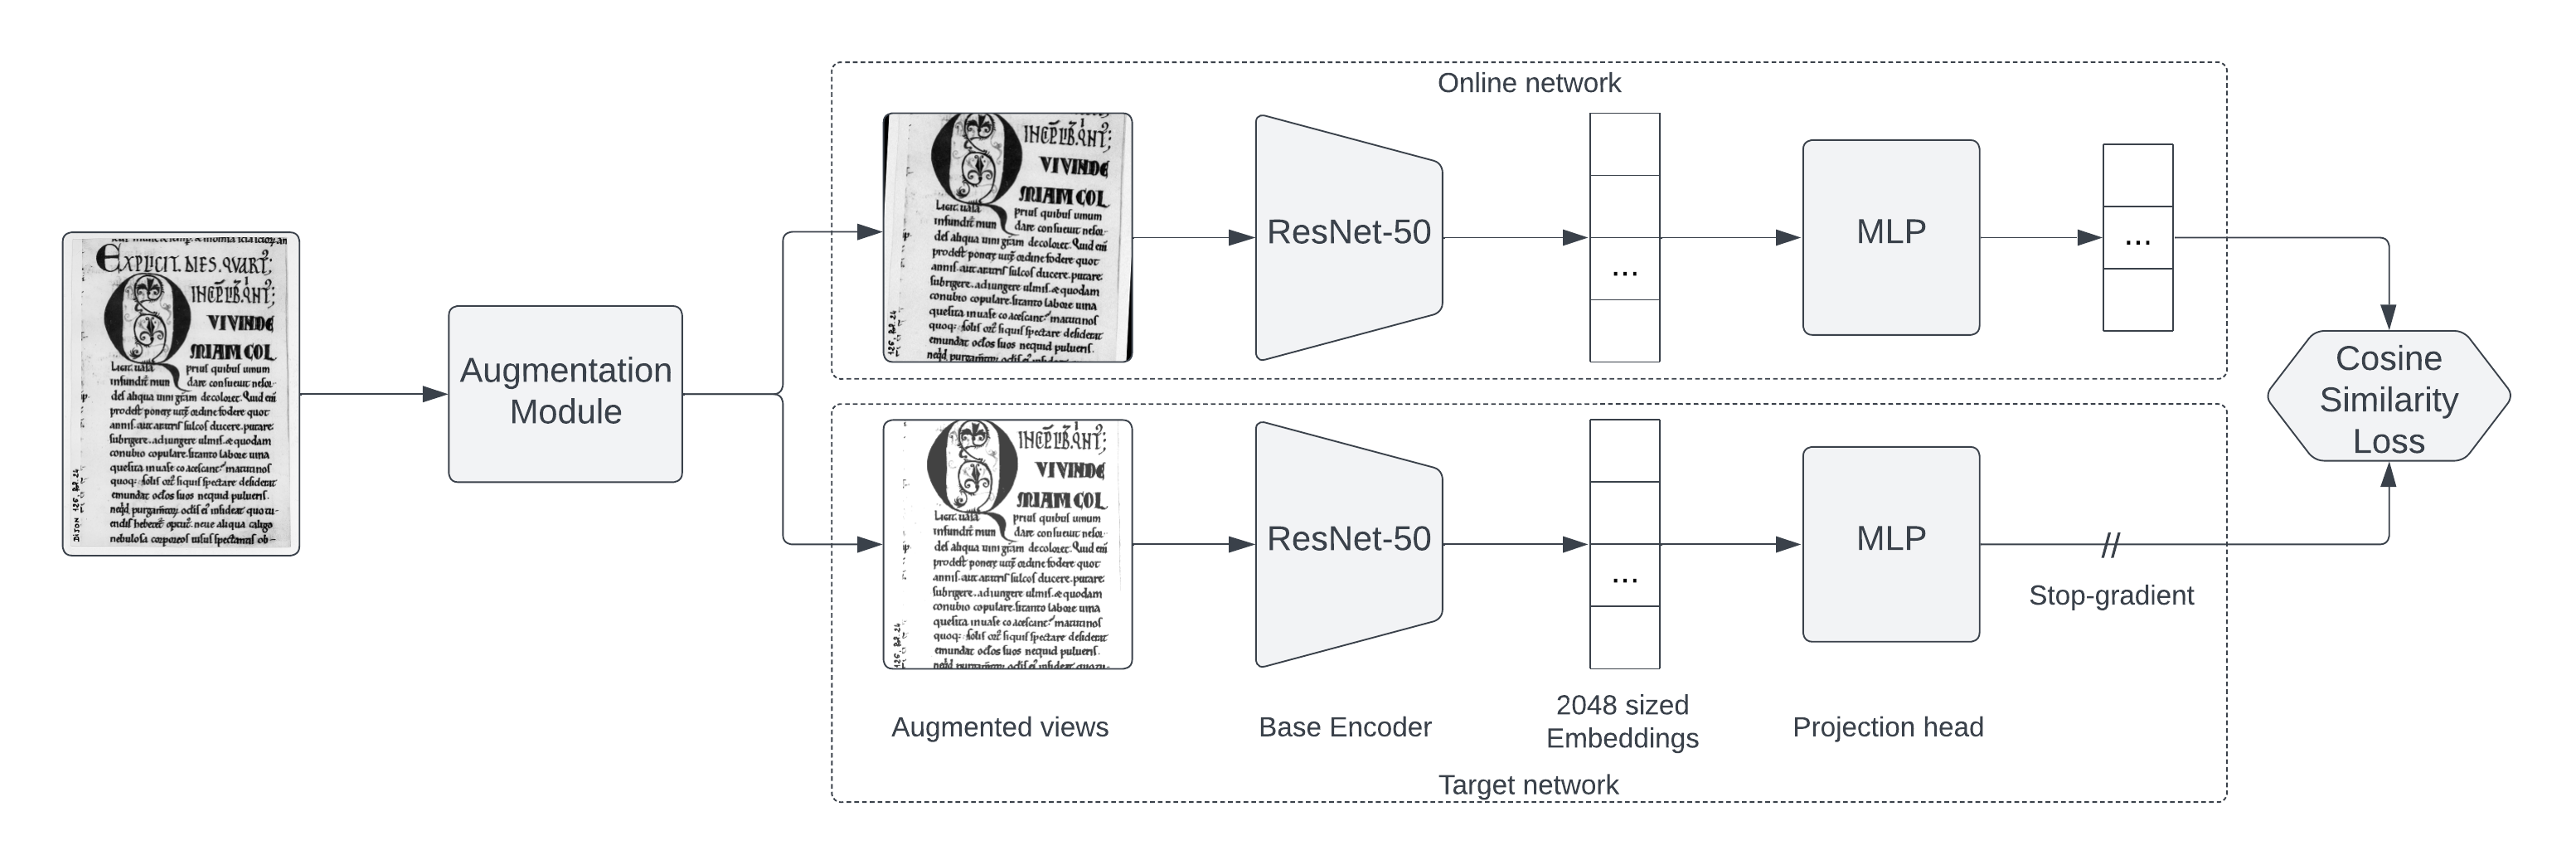
\includegraphics[width=\textwidth]{byol_arch.png}
\centering
\caption{BYOL Architecture}
\label{fig:figure}
\end{figure}
   % (\chapter{})

\chapter{Experimental setup and results}

The three self-supervised learning techniques mentioned were used in this study based on recommendations from the relevant research papers and with some customization. After training and evaluating these models using a linear evaluation protocol, it is concluded that the \gls{simclr} model outperforms the other methods mentioned given the setup. The following sections describe the model hyperparameter customizations, image transformations used, and a comparative analysis of the results.

\section{Model Configuration and Customizations}

The \gls{simclr} model includes erosion, dilation and random erasing in addition to transformations from Ying Chen et al. \cite{chen_simple_2020}. Each transform was applied randomly with a probability of 0.5. A kernel size of 5 is utilized for dilation while a kernel size of 3 is employed for erosion. An identical approach was used in \gls{byol} for preprocessing. The model configuration and hyperparameters passed for all the models are defined in \cref{tab:model-config}.

\begin{table}[ht]
	\begin{center}
            \caption{Pre-training configuration.}
		\resizebox{\textwidth}{!}{
			\begin{tabular}{@{}ll|ll|ll@{}}
				\toprule
				\multicolumn{2}{c|}{SimCLR}              & \multicolumn{2}{c|}{MAE}                       & \multicolumn{2}{c}{BYOL}                            \\ \midrule
				Variable           & Value               & Variable           & Value              & Variable           & Value             \\ \midrule
				Optimizer          & Adam                & Optimizer          & AdamW              & Optimizer          & Adam              \\
				Base learning rate & 1.5e-3              & Base learning rate & 3e-4               & Base learning rate & 3e-1              \\
				Weight decay       & 1e-6                & Optimizer momentum & $\beta_1=0.9, \beta_2=0.95$  & Weight decay       & 1.5e-6            \\
				Batch size         & 256                 & Weight decay       & 5e-2               & Target decay rate  & 0.996             \\
				Scheduler          & LambdaLR            & Scheduler          & Half-cycle cosine  & Batch size         & 64                \\
				Scheduler Function & Linear warmup decay & Batch size         & 512                & Scheduler          & Cosine annealing  \\
				Warmup Epochs      & 10                  & Warmup Epochs      & 10                 & Warmup Epochs      & 10                \\
				Loss function      & NT-Xent             & Loss function      & MSE                & Loss function      & Cosine similarity \\
				Temperature        & 0.1                 & Backbone           & Vision Transformer & Backbone           & ResNet-50         \\
				Backbone           & ResNet-50           &                    &                    &                    &                   \\ \bottomrule
			\end{tabular}
		}
		\vspace{5pt}
		\label{tab:model-config}
	\end{center}
\end{table}

Evaluation of multiple \gls{vit} block sizes for backbone architecture in \gls{mae} revealed that ViT-Large demonstrated superior performance in terms of learning and numerical stability. Whereas, both ViT-Base and ViT-Huge consistently resulted in \gls{nan} loss, while ViT-Tiny proved to be insufficient to learn features. Whereas, the added Erosion and Dilation augmentations to SimCLR were not performing well. Furthermore, extensive experimentation revealed that a large batch size of 512 and a learning rate scheduler are crucial for attaining good training results.

\section{Pre-training progress and monitoring}

The self-supervised methods in this study are pre-trained on the \gls{icdar}-\gls{clamm} dataset, which encompasses 12 classes for script type classification. To ensure consistency and reproducibility, a deterministic train, validation, and test split is performed, with a ratio of 70:10:20 percentages and a seed of 42. The test set remains untouched and is reserved for subsequent evaluation.

The models are pre-trained for a total of 500 epochs. The choice of a larger number of epochs is driven by the fact that the models are trained from scratch. This extended training duration allows the models to learn meaningful representations and capture intricate patterns present in the dataset.

By utilizing the powerful computational capabilities of \glspl{gpu} and parallel data loading to accelerate the training process, resulting in the convergence of the models over 500 epochs. Over 150 experiments were conducted with varying configurations to find optimal parameters for convergence.

\begin{figure}[ht]
	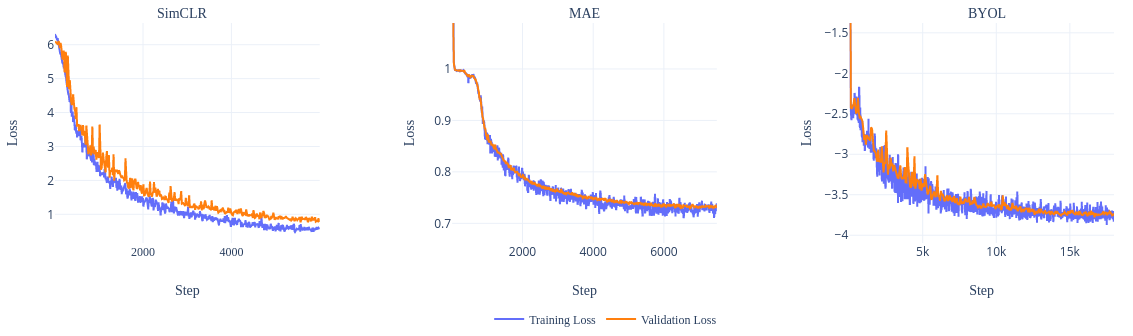
\includegraphics[width=\textwidth]{all_loss_curves.png}
	\centering
	\caption[Pre-training loss curves]{Loss curves for pre-trained models with batch size of 256, 256 and 64 from left to right.}
	\label{fig:loss}
\end{figure}

Throughout the pretraining process, periodic evaluations are conducted to monitor the models’ progress. Metrics such as training loss, validation loss, and grad norm are measured to assess the performance of the models at different stages of training. The loss curves for the best performing model generated during pre-training are shown in the \cref{fig:loss}. These metrics played a crucial role in identifying and mitigating \gls{nan} loss caused by the issues of vanishing and exploding gradients.

\begin{figure}
	\centering
	\begin{subfigure}[b]{0.3\textwidth}
		\centering
		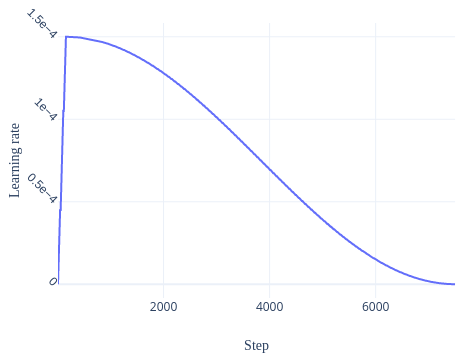
\includegraphics[width=\textwidth]{cosine_lr_sched.png}
		\caption{Learning rate}
	\end{subfigure}
	\hspace{10pt}
	\begin{subfigure}[b]{0.3\textwidth}
		\centering
		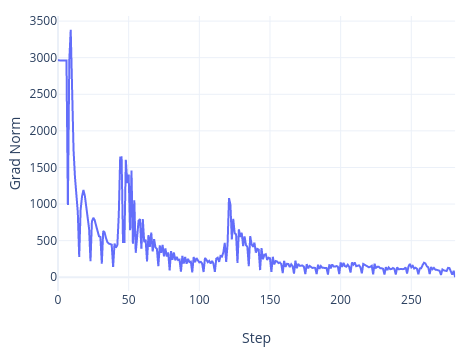
\includegraphics[width=\textwidth]{grad_norm.png}
		\caption{Normalized gradient}
	\end{subfigure}
	\caption[Metrics monitored for MAE]{Metrics for MAE (a) Half-cycle cosine learning rate decay after warmup. (b) Normalized gradient after each step.}
    \label{fig:lr_sched_grad}
\end{figure}

\section{Performance Evaluation}

In order to assess the effectiveness of the learned representations through transfer learning, a downstream task of script type classification is performed using the pre-trained models. This evaluation serves to gauge the transferability and generalization capabilities of the representations acquired during the self-supervised pretraining phase.

\subsection{Evaluation Metric}

To assess the quality and transferability of the learned representations, a linear evaluation protocol is employed. This evaluation protocol serves as a standardized framework for evaluating the performance of the pre-trained models on a downstream task \cite{kocaman_saliency_2022}. During the linear evaluation, the accuracy metric is employed to measure the performance of the linear classifier on the script type classification task. These metrics provide a quantitative assessment of the models’ ability to generalize and make accurate predictions in the specific task context.

In addition, to acquire insights into the class distribution and the quality of the learned embeddings, a visualization technique based on \acrfull{tsne} is employed. \gls{tsne} provides a powerful visualization method for exploring high-dimensional data by reducing its dimensionality while preserving the underlying structure \cite{maaten_visualizing_2008}.

\begin{figure}[ht]
	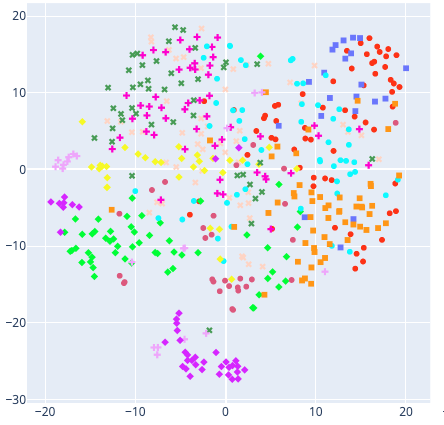
\includegraphics[width=0.45\textwidth]{simclr_embed_visualization.png}
	\centering
	\caption{t-SNE visualization of embeddings with 12 classes for SimCLR}
	\label{fig:figure}
\end{figure}


\subsection{Quantitative Results}

In this section, the results from the evaluations are presented and compared. The evaluation results for all the models are displayed in the \cref{tab:eval}. It is evident that, with a linear evaluation accuracy of 71.8\% \gls{simclr} outperforms \gls{mae} and \gls{byol}. 

\begin{table}[ht]
\begin{center}
\caption{Evaluation results.}
\begin{tabular}{@{}l|cc|cc@{}}
\multicolumn{1}{c|}{}       & \multicolumn{2}{c|}{Pre-training} & \multicolumn{2}{c}{Linear Evaluation}                                                                                 \\ \midrule
\multicolumn{1}{c|}{Model Name} & Epochs        & Batch size        & \begin{tabular}[c]{@{}c@{}}Training \\ epochs\end{tabular} & \begin{tabular}[c]{@{}c@{}}Top-1\\ accuracy\end{tabular} \\ \midrule
SimCLR                      & 500           & 256               & 100                                                        & 71.8\%                                                   \\
MAE                         & 500           & 256               & 100                                                        & 36.1\%                                                   \\
BYOL                        & 500           & 64                & 100                                                        & 45.2\%                                                  
\end{tabular}
\label{tab:eval}
\end{center}
\end{table}

It is worth noting that \gls{mae} with a \gls{vit} backbone shows a lower accuracy of 36.1\%. This observation can be attributed to its higher data requirements, as \gls{mae} with \gls{vit} demands a larger dataset for effective pre-training. The lower accuracy suggests that the available dataset size might not have been sufficient to fully leverage the potential of the \gls{mae} model with a \gls{vit} backbone. These findings highlight the importance of the choice of model architecture and the impact it has on the performance of downstream tasks given the complexity of the dataset. \gls{simclr}’s success can be attributed to its ability to learn robust representations even with a comparatively smaller dataset.

\subsection{Computational Efficiency}

The models performance differs in terms of trainable parameters, pre-training time, checkpoint size for the same GPU acceleration. \gls{simclr} has the fewest parameters and the smallest checkpoint size, while \gls{mae} has the shortest pre-training time and the largest parameters. This indicates that \gls{simclr} is the least complex of all. Consideration of these factors can be crucial in selecting the most suitable model based on the available computational resources.

Furthermore, the implementation of effective learning techniques like gradient accumulation proved to be useful in training models with bigger batch sizes that exceed the memory capacity limitation of \glspl{gpu}. \cref{tab:computational} presents a comprehensive analysis of the metrics that impact computational efficiency, allowing for easy comparison. 


\begin{table}[ht]
\begin{center}
\caption{Comparison of computational efficiency metrics for models trained for 500 epochs.}
\begin{tabular}{@{}l|c|c|c|c@{}}
\multicolumn{1}{c|}{Model Name} & \begin{tabular}[c]{@{}c@{}}Trainable Params \\ (millions)\end{tabular} & \begin{tabular}[c]{@{}c@{}}Pre-training Time\\ (hours)\end{tabular} & GPU      & \begin{tabular}[c]{@{}c@{}}Checkpoint Size\\ (MB)\end{tabular} \\ \midrule
SimCLR                          & 30                     
& 4.3                                                                 & 1 x A100 & 329                                                            \\
MAE                             & 329                                                                    & 2.61                                                                & 1 x A100 & 3700                                                           \\
BYOL                            & 68                                                                     & 5.06                                                                & 1 x A100 & 528                                                           
\end{tabular}
\label{tab:computational}
\end{center}
\end{table}   % (\chapter{})

%% ... more chapters ....
\chapter{Conclusion}

Self-supervised image representation learning using deep convolutional neural networks and transformers for unlabelled data has shown great success. This project has extensively experimented on reviewing some of the state-of-the-art Self-supervised learning techniques on the \gls{icdar} \gls{clamm} dataset. Under the linear evaluation protocol on the dataset, \gls{simclr} performs the best among \gls{mae} and \gls{byol}, while using comparatively fewer parameters. In order to enhance accuracies, it is imperative to conduct further research and experimentation to delve into the intricacies of \gls{mae} and \gls{byol} methodologies. Nevertheless, this study will be the foundation for implementing Self-supervised techniques for learning good representations in ancient handwritten script data.   % Conclusion (\chapter{Conclusion}  TEXT)
%\cleardoublepage

\appendix
\cleardoublepage

   % appendix A
\cleardoublepage
%\include{thesis10}   % appendix B
%\cleardoublepage
%\include{thesis11}   % appendix C
%\cleardoublepage

%% Do not change, auto-generated lists of figures, tables and literature %%
% Glossar
\printunsrtglossary[type=abbreviations]
\cleardoublepage

% List of figures
\addcontentsline{toc}{chapter}{\listfigurename}
\listoffigures
\cleardoublepage

% List of tables
\addcontentsline{toc}{chapter}{\listtablename}
\listoftables
\cleardoublepage

% Literature list
% %CONFIG:
%\selectlanguage{german}{\addcontentsline{toc}{chapter}{\bibname}}
\selectlanguage{english}{\addcontentsline{toc}{chapter}{\bibname}}

\printbibliography
\end{document}
